% ##################################################################################################################
\chapter{Aliaga}
\label{ch:aliaga}
\hfill \textbf{Authors:} Pelin Onelcin,Mehmet Metin Mutlu, Yalcin Alver

% ##################################################################################################################
Aliaga is one of the 30\,districts of Izmir Province in the Aegean Region of Turkey. 
The town is situated in about 50\,kilometers north of Izmir and has crucial contributions to Turkey’s economy. 
Aliaga has one of the greatest petrochemical enterprises of Turkey, called Petkim, In~2011, Petkim was ranked as the 12th greatest enterprise among 500\,top industrial enterprises in Turkey \citep[][]{}(Istanbul Chamber of Industry, 2011). There are 14\,plants and seven auxiliary units belonging to Petkim. 

Turkish Statistical Institute announces the population of Aliaga as 68\,432 among which 56\,440 live in the central neighborhoods and 11\,992 live in the villages in year~2011 \citep[][]{} (Turkish Statistical Institute, 2011).

There are many chemical factories located near the residential areas. The evacuation zone is determined based on a scenario developed for a chemical accident in one of the factories of Petkim. Features of the chemical substances and the National Fire Protection Association (NFPA~704) ratings ranging from 1 to 4, given for flammability, health and reactivity are compared. The most dangerous substance is acrylonitrile (ACN) with the ratings 3, 4, 2 for flammability, health and reactivity, respectively.

The radius of the risk zones are found via Aloha software developed by Office of Emergency Management and Emergency Response Division. The software divided the risk area into three zones based on the type of the chemical substance, wind speed and wind direction. The wind data obtained from Aliaga wind measurement station shows that the maximum wind speed is 17\,meters per second \citep[][]{}(WolframAlpha, 2012) and the prevailing wind direction is WNW. The wind blowing from west is the most dangerous one for Aliaga, because it would carry the smoke over residential areas which would increase the number of persons to be evacuated.

The evacuation zone is divided into 19\,\glspl{taz}. The trips that are generated from these zones are directed to six destination \glspl{taz} of which three of them are health care centers and three of them are gathering-places. Petkim area is divided into six zones where the first zone is in the impact area. In Figure~\ref{fig:aliaga_fig1} evacuation planning zone is shown.

Number of evacuees is calculated considering the permanent residents and employees being as transients. The scenario is prepared by taking into account the following conditions:
%
\begin{itemize}\styleItemize
\item The explosion occurs in the evening when there are no students in schools and people are awake.
%
\item The employees in the first risk zone and partially in the second risk zone are taken to the Aliaga state hospital in zone~30, and to the other health care centers in zones~26 and~27. The first risk zone is the most vulnerable zone, thus, persons who need medical intervention in this area should be taken to hospital. The typical behavior of persons in Turkey is to flock to hospitals in emergency situations. In generation of the scenarios this behavior is considered and not only in the first risk zone but also in the second risk zone health care centers are determined as destination zones.
%
\item People living in the residential zones self-evacuate. Since Aliaga is a small town, public transportation service is weak. Moreover, in the evening the frequency of public transportation is low. Therefore, public transportation is not considered in the present study.
%
\item The employees in Petkim and in Tupras work in three shifts. The factories are active for 24\,hours and there always are employees present in the factories.
\end{itemize}

The total number of the employees in the studied area is 3\,883. The number of employees to be evacuated from the factories is computed by means of the following assumptions:
%
\begin{itemize}\styleItemize
\item The total number of the employees is divided into three as they work in three shifts.
%
\item The time of the explosion does not correspond to the time of the shift change.
\end{itemize}

The number of evacuees from the residential buildings is calculated following these steps:
%
\begin{itemize}\styleItemize
\item The number of the persons living in the neighborhood belonging to the evacuation zone is divided into the number of the buildings in that neighborhood which give the mean number of the persons living in one building.
%
\item The number of the buildings that remains in the evacuation zone is multiplied by the mean number of persons in one building.
\end{itemize}

Here, to estimate the number of evacuation vehicles, car occupancy ratio rate is used. This rate is 1.57 in normal situations \citep[][]{}(Istanbul Metropolitan Municipality Directorate of Transportation Planning, 2011) however in emergency situation it is expected to be higher. In this study the car occupancy ratio rate is taken as two. The number of evacuees is computed as 14\,472 and the number of vehicles is computed as 7\,236.

The network of Aliaga has been taken from \gls{osm} and has been converted to a shape file and \gls{matsim} network file with \lstinline|NetworkGenerator| class of \gls{matsim}. Zones used in generating synthetic population for \gls{matsim} were created in Quantum GIS (QGIS).

Three different scenarios have been identified for the evacuation simulation. In Table~\ref{tab:aliaga_tab1}1, \gls{od} matrices for each scenario can be seen. The selection of these three scenarios is mainly based on the location of the destination zones and traffic demand. Free spaces which are close to the risk zone are designated as gathering-areas. The time required for the evacuees to reach health care centers is of significant importance in an emergency situation such as in this case. The traffic demand generated for the health care centers is distributed between zone~26, 27 and~30 in the scenarios though the first risk zone is always directed to Aliaga State Hospital for it has the greatest capacity among the health care centers and severely injured persons should be transferred to this state hospital. Evacuating vehicles departing from the second risk zone are directed to health care centers in zone~26 and~27. Changing the number of evacuating vehicles between these zones result in different evacuation times. Thus, these different scenarios could allow observing the effect of traffic demand on traffic and if this leads to any reduction in evacuation time.

Initial demand refers to synthetic population derived from numbers and locations of evacuees to be transferred to presumed health care centers or gathering-areas according to distance. \lstinline|DemandGenerator| module of \gls{matsim} \ah{?} is used to generate initial demand, which generates given zone. Zones are modified according to density of population that actually exists in given zone and road links that evacuees will possibly start their trip at a possible chemical accident moment to generate a relatively realistic scenario. The population zones are set for a group of origin zones which are assigned for a predefined destination. For each agent, random activity coordinates are generated such as home, work, and leisure or in this case evacuation zones and hospitals gathering areas. Departures and arrivals of the agents take place on the nodes which are closest to the activity coordinates, and in the first iteration shortest path is calculated for route choice.

\gls{matsim} assigns the trip start to closest node to coordinates of agent activity (\ie home or work) for each agent. Simulation results of \gls{matsim} are analyzed by \gls{senozon} \gls{via}. In Figure~\ref{fig:aliaga_fig2} a snapshot from the simulation is shown.

The clearance time of three risk zones and total arrival time for three different scenarios are listed in Table~\ref{tab:aliaga_tab2}. For the first scenario the evacuation times are 45\,minutes for the first risk zone, 83\,minutes for the second risk zone, and 86\,minutes for the third risk zone. For the second scenario the evacuation times are 44\,minutes for the first risk zone, 82\,minutes for the second risk zone, and 91\,minutes for the third risk zone. Finally, for the third scenario the evacuation times are 47\,minutes for the first risk zone, 86\,minutes for the second risk zone, and 88\,minutes for the third risk zone. The third scenario gives the best results with the minimum clearance time of the entire risk area among the given scenarios. Scenario results show us clearance times are not enough for people to evacuate safely, especially in the first risk zone.

% ##################################################################################################################

 % ------------
\createfigure%
{Evacuation planning zone}%
{Evacuation planning zone}%
{\label{fig:aliaga_fig1}}%
{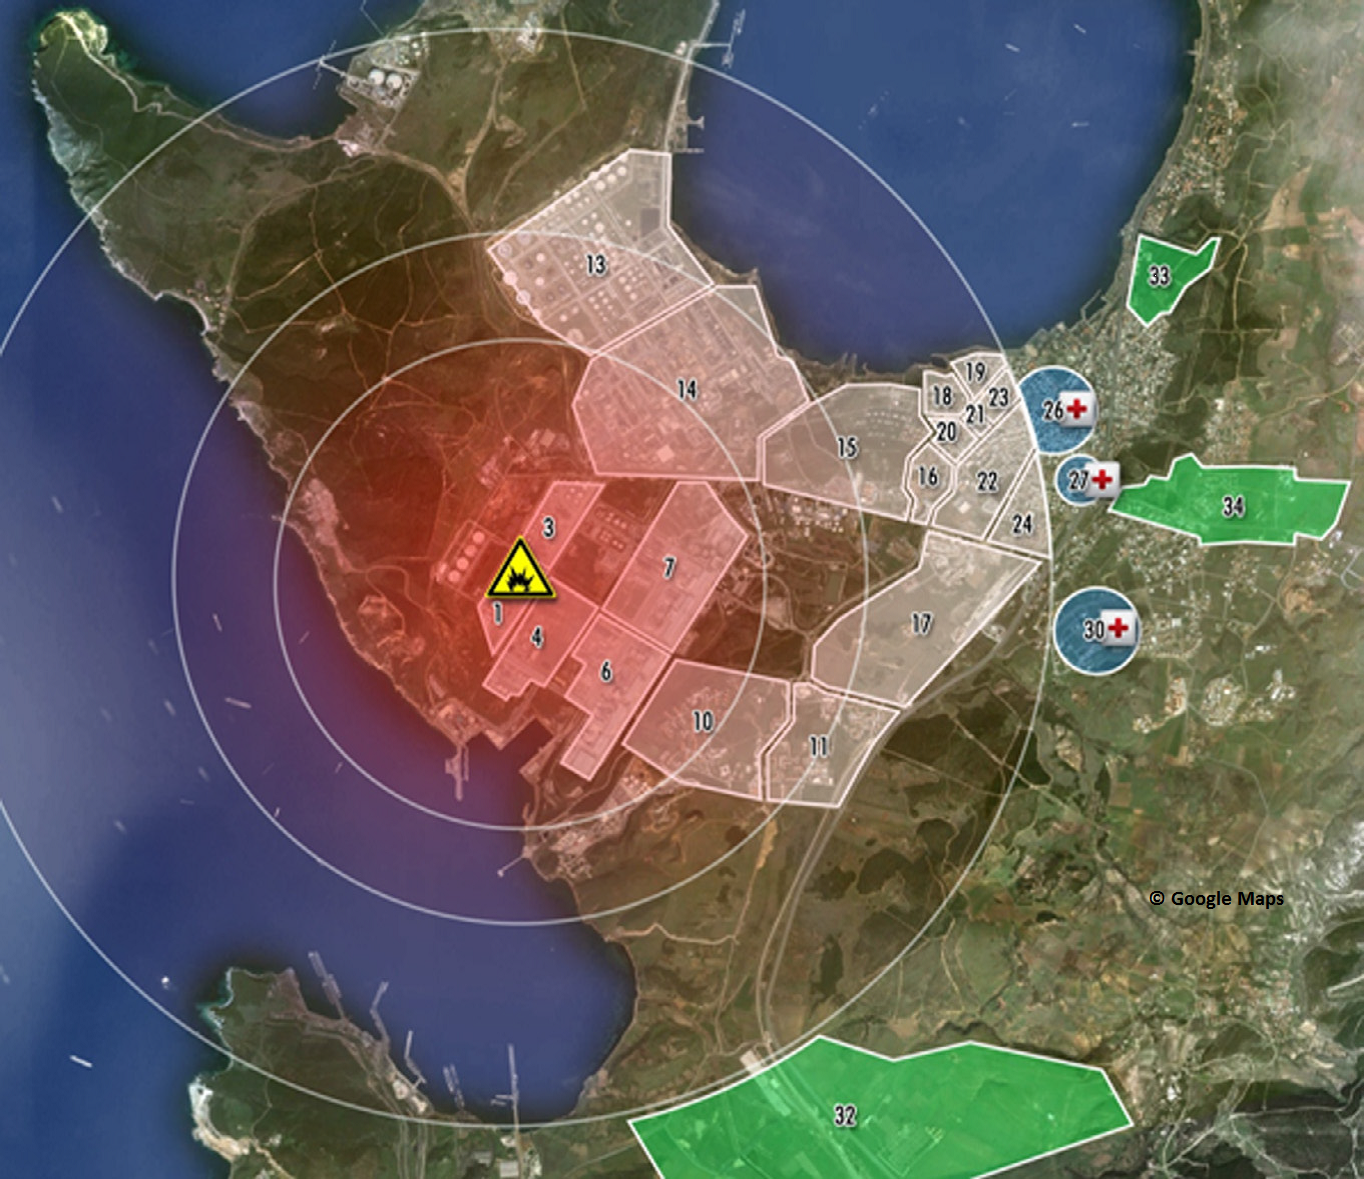
\includegraphics[width=0.8\textwidth, angle=0]{scenarios/figures/aliaga_fig1.png}}%
{}
% ------------

 % ------------
\createfigure%
{MATSim simulation snapshot}%
{MATSim simulation snapshot}%
{\label{fig:aliaga_fig2}}%
{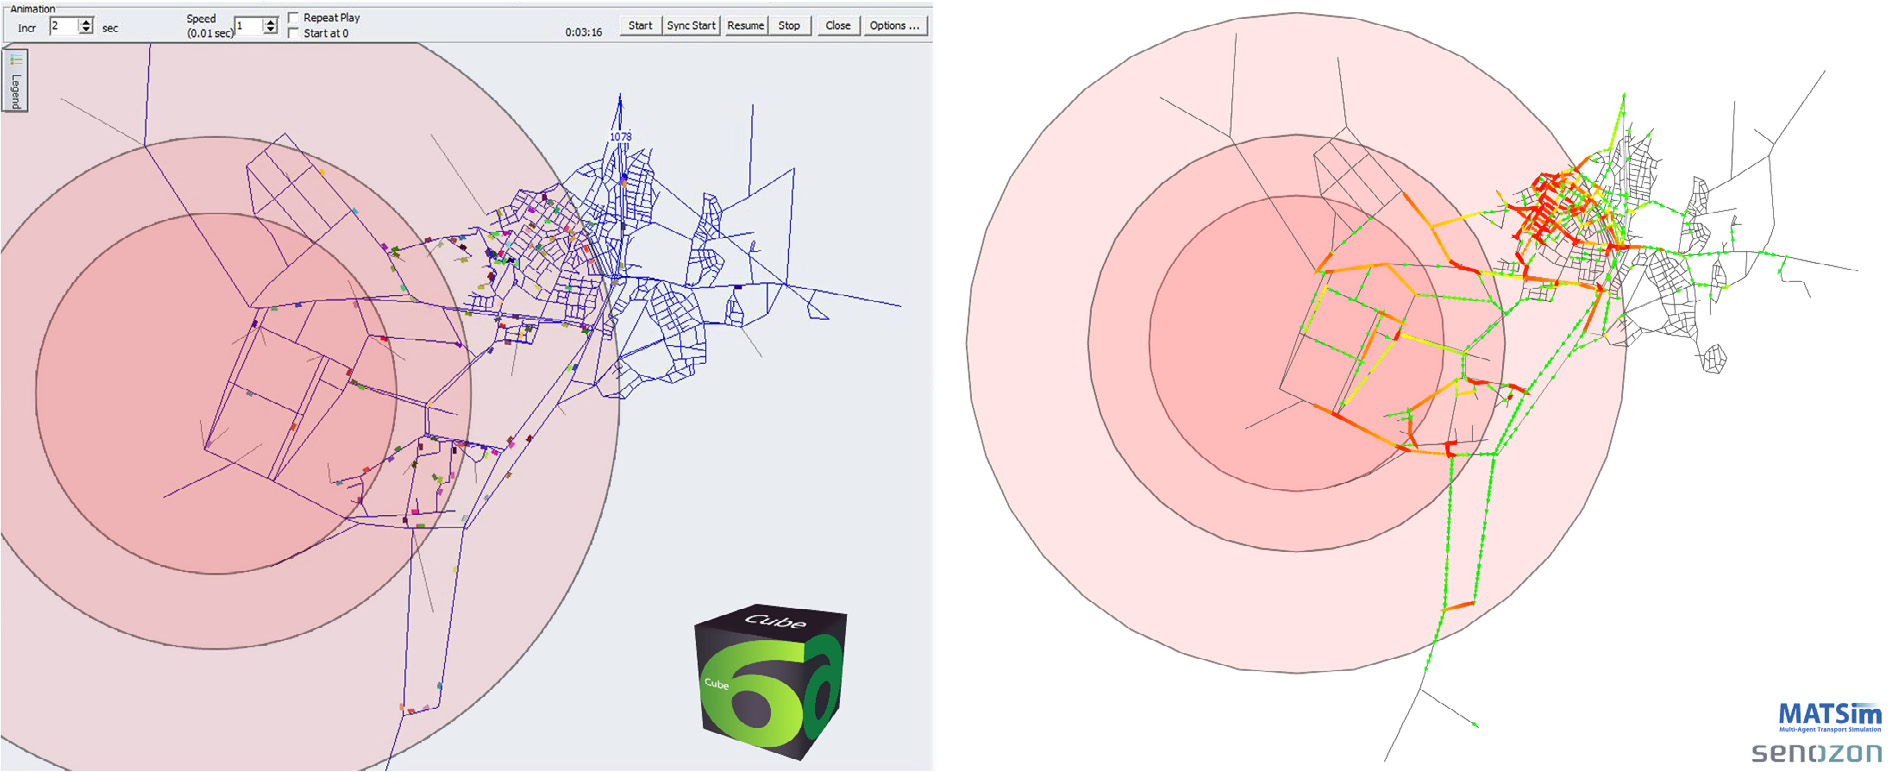
\includegraphics[width=0.8\textwidth, angle=0]{scenarios/figures/aliaga_fig2.png}}%
{}
% ------------

%---------------------------------------------------------------------
\createtable%
{Risk zones evacuation times in minutes}%
{Risk zones evacuation times in minutes}%
{\label{tab:aliaga_tab2}}%
{%
  \begin{tabular}[c]{|l|c|c|c|}
    \hline
		& \textbf{Risk zone~1} & \textbf{Risk zone~2} & \textbf{Risk zone~3} \\
		\hline
    Scenario~1 & 45 & 83 & 86 \\
		Scenario~2 & 44 & 82 & 91 \\
		Scenario~3 & 47 & 86 & 88 \\
    \hline
  \end{tabular}
}%
{}
%---------------------------------------------------------------------

% ##################################################################################################################
